
\documentclass{report}


%%%%%%%%%%%%%%%%%%%%%%%%%%%%%%%%%
% PACKAGE IMPORTS
%%%%%%%%%%%%%%%%%%%%%%%%%%%%%%%%%


\usepackage[tmargin=2cm,rmargin=1in,lmargin=1in,margin=0.85in,bmargin=2cm,footskip=.2in]{geometry}
\usepackage{amsmath,amsfonts,amsthm,amssymb,mathtools}
\usepackage[varbb]{newpxmath}
\usepackage{xfrac}
\usepackage[makeroom]{cancel}
\usepackage{mathtools}
\usepackage{bookmark}
\usepackage{enumitem}
\usepackage{hyperref,theoremref}
\hypersetup{
	pdftitle={Assignment},
	colorlinks=true, linkcolor=doc!90,
	bookmarksnumbered=true,
	bookmarksopen=true
}
\usepackage[most,many,breakable]{tcolorbox}
\usepackage{xcolor}
\usepackage{varwidth}
\usepackage{varwidth}
\usepackage{etoolbox}
%\usepackage{authblk}
\usepackage{nameref}
\usepackage{multicol,array}
\usepackage{tikz-cd}
\usepackage[ruled,vlined,linesnumbered]{algorithm2e}
\usepackage{comment} % enables the use of multi-line comments (\ifx \fi) 
\usepackage{import}
\usepackage{xifthen}
\usepackage{pdfpages}
\usepackage{transparent}

\newcommand\mycommfont[1]{\footnotesize\ttfamily\textcolor{blue}{#1}}
\SetCommentSty{mycommfont}
\newcommand{\incfig}[1]{%
    \def\svgwidth{\columnwidth}
    \import{./figures/}{#1.pdf_tex}
}

\usepackage{tikzsymbols}
\renewcommand\qedsymbol{$\Laughey$}


%\usepackage{import}
%\usepackage{xifthen}
%\usepackage{pdfpages}
%\usepackage{transparent}


%%%%%%%%%%%%%%%%%%%%%%%%%%%%%%
% SELF MADE COLORS
%%%%%%%%%%%%%%%%%%%%%%%%%%%%%%



\definecolor{myg}{RGB}{56, 140, 70}
\definecolor{myb}{RGB}{45, 111, 177}
\definecolor{myr}{RGB}{199, 68, 64}
\definecolor{mytheorembg}{HTML}{F2F2F9}
\definecolor{mytheoremfr}{HTML}{00007B}
\definecolor{mylenmabg}{HTML}{FFFAF8}
\definecolor{mylenmafr}{HTML}{983b0f}
\definecolor{mypropbg}{HTML}{f2fbfc}
\definecolor{mypropfr}{HTML}{191971}
\definecolor{myexamplebg}{HTML}{F2FBF8}
\definecolor{myexamplefr}{HTML}{88D6D1}
\definecolor{myexampleti}{HTML}{2A7F7F}
\definecolor{mydefinitbg}{HTML}{E5E5FF}
\definecolor{mydefinitfr}{HTML}{3F3FA3}
\definecolor{notesgreen}{RGB}{0,162,0}
\definecolor{myp}{RGB}{197, 92, 212}
\definecolor{mygr}{HTML}{2C3338}
\definecolor{myred}{RGB}{127,0,0}
\definecolor{myyellow}{RGB}{169,121,69}
\definecolor{myexercisebg}{HTML}{F2FBF8}
\definecolor{myexercisefg}{HTML}{88D6D1}


%%%%%%%%%%%%%%%%%%%%%%%%%%%%
% TCOLORBOX SETUPS
%%%%%%%%%%%%%%%%%%%%%%%%%%%%

\setlength{\parindent}{1cm}
%================================
% THEOREM BOX
%================================

\tcbuselibrary{theorems,skins,hooks}
\newtcbtheorem[number within=section]{Theorem}{Theorem}
{%
	enhanced,
	breakable,
	colback = mytheorembg,
	frame hidden,
	boxrule = 0sp,
	borderline west = {2pt}{0pt}{mytheoremfr},
	sharp corners,
	detach title,
	before upper = \tcbtitle\par\smallskip,
	coltitle = mytheoremfr,
	fonttitle = \bfseries\sffamily,
	description font = \mdseries,
	separator sign none,
	segmentation style={solid, mytheoremfr},
}
{th}

\tcbuselibrary{theorems,skins,hooks}
\newtcbtheorem[number within=chapter]{theorem}{Theorem}
{%
	enhanced,
	breakable,
	colback = mytheorembg,
	frame hidden,
	boxrule = 0sp,
	borderline west = {2pt}{0pt}{mytheoremfr},
	sharp corners,
	detach title,
	before upper = \tcbtitle\par\smallskip,
	coltitle = mytheoremfr,
	fonttitle = \bfseries\sffamily,
	description font = \mdseries,
	separator sign none,
	segmentation style={solid, mytheoremfr},
}
{th}


\tcbuselibrary{theorems,skins,hooks}
\newtcolorbox{Theoremcon}
{%
	enhanced
	,breakable
	,colback = mytheorembg
	,frame hidden
	,boxrule = 0sp
	,borderline west = {2pt}{0pt}{mytheoremfr}
	,sharp corners
	,description font = \mdseries
	,separator sign none
}

%================================
% Corollery
%================================
\tcbuselibrary{theorems,skins,hooks}
\newtcbtheorem[number within=section]{Corollary}{Corollary}
{%
	enhanced
	,breakable
	,colback = myp!10
	,frame hidden
	,boxrule = 0sp
	,borderline west = {2pt}{0pt}{myp!85!black}
	,sharp corners
	,detach title
	,before upper = \tcbtitle\par\smallskip
	,coltitle = myp!85!black
	,fonttitle = \bfseries\sffamily
	,description font = \mdseries
	,separator sign none
	,segmentation style={solid, myp!85!black}
}
{th}
\tcbuselibrary{theorems,skins,hooks}
\newtcbtheorem[number within=chapter]{corollary}{Corollary}
{%
	enhanced
	,breakable
	,colback = myp!10
	,frame hidden
	,boxrule = 0sp
	,borderline west = {2pt}{0pt}{myp!85!black}
	,sharp corners
	,detach title
	,before upper = \tcbtitle\par\smallskip
	,coltitle = myp!85!black
	,fonttitle = \bfseries\sffamily
	,description font = \mdseries
	,separator sign none
	,segmentation style={solid, myp!85!black}
}
{th}


%================================
% LENMA
%================================

\tcbuselibrary{theorems,skins,hooks}
\newtcbtheorem[number within=section]{Lenma}{Lenma}
{%
	enhanced,
	breakable,
	colback = mylenmabg,
	frame hidden,
	boxrule = 0sp,
	borderline west = {2pt}{0pt}{mylenmafr},
	sharp corners,
	detach title,
	before upper = \tcbtitle\par\smallskip,
	coltitle = mylenmafr,
	fonttitle = \bfseries\sffamily,
	description font = \mdseries,
	separator sign none,
	segmentation style={solid, mylenmafr},
}
{th}

\tcbuselibrary{theorems,skins,hooks}
\newtcbtheorem[number within=chapter]{lenma}{Lenma}
{%
	enhanced,
	breakable,
	colback = mylenmabg,
	frame hidden,
	boxrule = 0sp,
	borderline west = {2pt}{0pt}{mylenmafr},
	sharp corners,
	detach title,
	before upper = \tcbtitle\par\smallskip,
	coltitle = mylenmafr,
	fonttitle = \bfseries\sffamily,
	description font = \mdseries,
	separator sign none,
	segmentation style={solid, mylenmafr},
}
{th}


%================================
% PROPOSITION
%================================

\tcbuselibrary{theorems,skins,hooks}
\newtcbtheorem[number within=section]{Prop}{Proposition}
{%
	enhanced,
	breakable,
	colback = mypropbg,
	frame hidden,
	boxrule = 0sp,
	borderline west = {2pt}{0pt}{mypropfr},
	sharp corners,
	detach title,
	before upper = \tcbtitle\par\smallskip,
	coltitle = mypropfr,
	fonttitle = \bfseries\sffamily,
	description font = \mdseries,
	separator sign none,
	segmentation style={solid, mypropfr},
}
{th}

\tcbuselibrary{theorems,skins,hooks}
\newtcbtheorem[number within=chapter]{prop}{Proposition}
{%
	enhanced,
	breakable,
	colback = mypropbg,
	frame hidden,
	boxrule = 0sp,
	borderline west = {2pt}{0pt}{mypropfr},
	sharp corners,
	detach title,
	before upper = \tcbtitle\par\smallskip,
	coltitle = mypropfr,
	fonttitle = \bfseries\sffamily,
	description font = \mdseries,
	separator sign none,
	segmentation style={solid, mypropfr},
}
{th}


%================================
% CLAIM
%================================

\tcbuselibrary{theorems,skins,hooks}
\newtcbtheorem[number within=section]{claim}{Claim}
{%
	enhanced
	,breakable
	,colback = myg!10
	,frame hidden
	,boxrule = 0sp
	,borderline west = {2pt}{0pt}{myg}
	,sharp corners
	,detach title
	,before upper = \tcbtitle\par\smallskip
	,coltitle = myg!85!black
	,fonttitle = \bfseries\sffamily
	,description font = \mdseries
	,separator sign none
	,segmentation style={solid, myg!85!black}
}
{th}



%================================
% Exercise
%================================

\tcbuselibrary{theorems,skins,hooks}
\newtcbtheorem[number within=section]{Exercise}{Exercise}
{%
	enhanced,
	breakable,
	colback = myexercisebg,
	frame hidden,
	boxrule = 0sp,
	borderline west = {2pt}{0pt}{myexercisefg},
	sharp corners,
	detach title,
	before upper = \tcbtitle\par\smallskip,
	coltitle = myexercisefg,
	fonttitle = \bfseries\sffamily,
	description font = \mdseries,
	separator sign none,
	segmentation style={solid, myexercisefg},
}
{th}

\tcbuselibrary{theorems,skins,hooks}
\newtcbtheorem[number within=chapter]{exercise}{Exercise}
{%
	enhanced,
	breakable,
	colback = myexercisebg,
	frame hidden,
	boxrule = 0sp,
	borderline west = {2pt}{0pt}{myexercisefg},
	sharp corners,
	detach title,
	before upper = \tcbtitle\par\smallskip,
	coltitle = myexercisefg,
	fonttitle = \bfseries\sffamily,
	description font = \mdseries,
	separator sign none,
	segmentation style={solid, myexercisefg},
}
{th}

%================================
% EXAMPLE BOX
%================================

\newtcbtheorem[number within=section]{Example}{Example}
{%
	colback = myexamplebg
	,breakable
	,colframe = myexamplefr
	,coltitle = myexampleti
	,boxrule = 1pt
	,sharp corners
	,detach title
	,before upper=\tcbtitle\par\smallskip
	,fonttitle = \bfseries
	,description font = \mdseries
	,separator sign none
	,description delimiters parenthesis
}
{ex}

\newtcbtheorem[number within=chapter]{example}{Example}
{%
	colback = myexamplebg
	,breakable
	,colframe = myexamplefr
	,coltitle = myexampleti
	,boxrule = 1pt
	,sharp corners
	,detach title
	,before upper=\tcbtitle\par\smallskip
	,fonttitle = \bfseries
	,description font = \mdseries
	,separator sign none
	,description delimiters parenthesis
}
{ex}

%================================
% DEFINITION BOX
%================================

\newtcbtheorem[number within=section]{Definition}{Definition}{enhanced,
	before skip=2mm,after skip=2mm, colback=red!5,colframe=red!80!black,boxrule=0.5mm,
	attach boxed title to top left={xshift=1cm,yshift*=1mm-\tcboxedtitleheight}, varwidth boxed title*=-3cm,
	boxed title style={frame code={
					\path[fill=tcbcolback]
					([yshift=-1mm,xshift=-1mm]frame.north west)
					arc[start angle=0,end angle=180,radius=1mm]
					([yshift=-1mm,xshift=1mm]frame.north east)
					arc[start angle=180,end angle=0,radius=1mm];
					\path[left color=tcbcolback!60!black,right color=tcbcolback!60!black,
						middle color=tcbcolback!80!black]
					([xshift=-2mm]frame.north west) -- ([xshift=2mm]frame.north east)
					[rounded corners=1mm]-- ([xshift=1mm,yshift=-1mm]frame.north east)
					-- (frame.south east) -- (frame.south west)
					-- ([xshift=-1mm,yshift=-1mm]frame.north west)
					[sharp corners]-- cycle;
				},interior engine=empty,
		},
	fonttitle=\bfseries,
	title={#2},#1}{def}
\newtcbtheorem[number within=chapter]{definition}{Definition}{enhanced,
	before skip=2mm,after skip=2mm, colback=red!5,colframe=red!80!black,boxrule=0.5mm,
	attach boxed title to top left={xshift=1cm,yshift*=1mm-\tcboxedtitleheight}, varwidth boxed title*=-3cm,
	boxed title style={frame code={
					\path[fill=tcbcolback]
					([yshift=-1mm,xshift=-1mm]frame.north west)
					arc[start angle=0,end angle=180,radius=1mm]
					([yshift=-1mm,xshift=1mm]frame.north east)
					arc[start angle=180,end angle=0,radius=1mm];
					\path[left color=tcbcolback!60!black,right color=tcbcolback!60!black,
						middle color=tcbcolback!80!black]
					([xshift=-2mm]frame.north west) -- ([xshift=2mm]frame.north east)
					[rounded corners=1mm]-- ([xshift=1mm,yshift=-1mm]frame.north east)
					-- (frame.south east) -- (frame.south west)
					-- ([xshift=-1mm,yshift=-1mm]frame.north west)
					[sharp corners]-- cycle;
				},interior engine=empty,
		},
	fonttitle=\bfseries,
	title={#2},#1}{def}



%================================
% Solution BOX
%================================

\makeatletter
\newtcbtheorem{question}{Question}{enhanced,
	breakable,
	colback=white,
	colframe=myb!80!black,
	attach boxed title to top left={yshift*=-\tcboxedtitleheight},
	fonttitle=\bfseries,
	title={#2},
	boxed title size=title,
	boxed title style={%
			sharp corners,
			rounded corners=northwest,
			colback=tcbcolframe,
			boxrule=0pt,
		},
	underlay boxed title={%
			\path[fill=tcbcolframe] (title.south west)--(title.south east)
			to[out=0, in=180] ([xshift=5mm]title.east)--
			(title.center-|frame.east)
			[rounded corners=\kvtcb@arc] |-
			(frame.north) -| cycle;
		},
	#1
}{def}
\makeatother

%================================
% SOLUTION BOX
%================================

\makeatletter
\newtcolorbox{solution}{enhanced,
	breakable,
	colback=white,
	colframe=myg!80!black,
	attach boxed title to top left={yshift*=-\tcboxedtitleheight},
	title=Solution,
	boxed title size=title,
	boxed title style={%
			sharp corners,
			rounded corners=northwest,
			colback=tcbcolframe,
			boxrule=0pt,
		},
	underlay boxed title={%
			\path[fill=tcbcolframe] (title.south west)--(title.south east)
			to[out=0, in=180] ([xshift=5mm]title.east)--
			(title.center-|frame.east)
			[rounded corners=\kvtcb@arc] |-
			(frame.north) -| cycle;
		},
}
\makeatother

%================================
% Question BOX
%================================

\makeatletter
\newtcbtheorem{qstion}{Question}{enhanced,
	breakable,
	colback=white,
	colframe=mygr,
	attach boxed title to top left={yshift*=-\tcboxedtitleheight},
	fonttitle=\bfseries,
	title={#2},
	boxed title size=title,
	boxed title style={%
			sharp corners,
			rounded corners=northwest,
			colback=tcbcolframe,
			boxrule=0pt,
		},
	underlay boxed title={%
			\path[fill=tcbcolframe] (title.south west)--(title.south east)
			to[out=0, in=180] ([xshift=5mm]title.east)--
			(title.center-|frame.east)
			[rounded corners=\kvtcb@arc] |-
			(frame.north) -| cycle;
		},
	#1
}{def}
\makeatother

\newtcbtheorem[number within=chapter]{wconc}{Wrong Concept}{
	breakable,
	enhanced,
	colback=white,
	colframe=myr,
	arc=0pt,
	outer arc=0pt,
	fonttitle=\bfseries\sffamily\large,
	colbacktitle=myr,
	attach boxed title to top left={},
	boxed title style={
			enhanced,
			skin=enhancedfirst jigsaw,
			arc=3pt,
			bottom=0pt,
			interior style={fill=myr}
		},
	#1
}{def}



%================================
% NOTE BOX
%================================

\usetikzlibrary{arrows,calc,shadows.blur}
\tcbuselibrary{skins}
\newtcolorbox{note}[1][]{%
	enhanced jigsaw,
	colback=gray!20!white,%
	colframe=gray!80!black,
	size=small,
	boxrule=1pt,
	title=\textbf{Note:-},
	halign title=flush center,
	coltitle=black,
	breakable,
	drop shadow=black!50!white,
	attach boxed title to top left={xshift=1cm,yshift=-\tcboxedtitleheight/2,yshifttext=-\tcboxedtitleheight/2},
	minipage boxed title=1.5cm,
	boxed title style={%
			colback=white,
			size=fbox,
			boxrule=1pt,
			boxsep=2pt,
			underlay={%
					\coordinate (dotA) at ($(interior.west) + (-0.5pt,0)$);
					\coordinate (dotB) at ($(interior.east) + (0.5pt,0)$);
					\begin{scope}
						\clip (interior.north west) rectangle ([xshift=3ex]interior.east);
						\filldraw [white, blur shadow={shadow opacity=60, shadow yshift=-.75ex}, rounded corners=2pt] (interior.north west) rectangle (interior.south east);
					\end{scope}
					\begin{scope}[gray!80!black]
						\fill (dotA) circle (2pt);
						\fill (dotB) circle (2pt);
					\end{scope}
				},
		},
	#1,
}

%%%%%%%%%%%%%%%%%%%%%%%%%%%%%%
% SELF MADE COMMANDS
%%%%%%%%%%%%%%%%%%%%%%%%%%%%%%


\newcommand{\thm}[2]{\begin{Theorem}{#1}{}#2\end{Theorem}}
\newcommand{\cor}[2]{\begin{Corollary}{#1}{}#2\end{Corollary}}
\newcommand{\mlenma}[2]{\begin{Lenma}{#1}{}#2\end{Lenma}}
\newcommand{\mprop}[2]{\begin{Prop}{#1}{}#2\end{Prop}}
\newcommand{\clm}[3]{\begin{claim}{#1}{#2}#3\end{claim}}
\newcommand{\wc}[2]{\begin{wconc}{#1}{}\setlength{\parindent}{1cm}#2\end{wconc}}
\newcommand{\thmcon}[1]{\begin{Theoremcon}{#1}\end{Theoremcon}}
\newcommand{\ex}[2]{\begin{Example}{#1}{}#2\end{Example}}
\newcommand{\dfn}[2]{\begin{Definition}[colbacktitle=red!75!black]{#1}{}#2\end{Definition}}
\newcommand{\dfnc}[2]{\begin{definition}[colbacktitle=red!75!black]{#1}{}#2\end{definition}}
\newcommand{\qs}[2]{\begin{question}{#1}{}#2\end{question}}
\newcommand{\pf}[2]{\begin{myproof}[#1]#2\end{myproof}}
\newcommand{\nt}[1]{\begin{note}#1\end{note}}

\newcommand*\circled[1]{\tikz[baseline=(char.base)]{
		\node[shape=circle,draw,inner sep=1pt] (char) {#1};}}
\newcommand\getcurrentref[1]{%
	\ifnumequal{\value{#1}}{0}
	{??}
	{\the\value{#1}}%
}
\newcommand{\getCurrentSectionNumber}{\getcurrentref{section}}
\newenvironment{myproof}[1][\proofname]{%
	\proof[\bfseries #1: ]%
}{\endproof}

\newcommand{\mclm}[2]{\begin{myclaim}[#1]#2\end{myclaim}}
\newenvironment{myclaim}[1][\claimname]{\proof[\bfseries #1: ]}{}

\newcounter{mylabelcounter}

\makeatletter
\newcommand{\setword}[2]{%
	\phantomsection
	#1\def\@currentlabel{\unexpanded{#1}}\label{#2}%
}
\makeatother




\tikzset{
	symbol/.style={
			draw=none,
			every to/.append style={
					edge node={node [sloped, allow upside down, auto=false]{$#1$}}}
		}
}


% deliminators
\DeclarePairedDelimiter{\abs}{\lvert}{\rvert}
\DeclarePairedDelimiter{\norm}{\lVert}{\rVert}

\DeclarePairedDelimiter{\ceil}{\lceil}{\rceil}
\DeclarePairedDelimiter{\floor}{\lfloor}{\rfloor}
\DeclarePairedDelimiter{\round}{\lfloor}{\rceil}

\newsavebox\diffdbox
\newcommand{\slantedromand}{{\mathpalette\makesl{d}}}
\newcommand{\makesl}[2]{%
\begingroup
\sbox{\diffdbox}{$\mathsurround=0pt#1\mathrm{#2}$}%
\pdfsave
\pdfsetmatrix{1 0 0.2 1}%
\rlap{\usebox{\diffdbox}}%
\pdfrestore
\hskip\wd\diffdbox
\endgroup
}
\newcommand{\dd}[1][]{\ensuremath{\mathop{}\!\ifstrempty{#1}{%
\slantedromand\@ifnextchar^{\hspace{0.2ex}}{\hspace{0.1ex}}}%
{\slantedromand\hspace{0.2ex}^{#1}}}}
\ProvideDocumentCommand\dv{o m g}{%
  \ensuremath{%
    \IfValueTF{#3}{%
      \IfNoValueTF{#1}{%
        \frac{\dd #2}{\dd #3}%
      }{%
        \frac{\dd^{#1} #2}{\dd #3^{#1}}%
      }%
    }{%
      \IfNoValueTF{#1}{%
        \frac{\dd}{\dd #2}%
      }{%
        \frac{\dd^{#1}}{\dd #2^{#1}}%
      }%
    }%
  }%
}
\providecommand*{\pdv}[3][]{\frac{\partial^{#1}#2}{\partial#3^{#1}}}
%  - others
\DeclareMathOperator{\Lap}{\mathcal{L}}
\DeclareMathOperator{\Var}{Var} % varience
\DeclareMathOperator{\Cov}{Cov} % covarience
\DeclareMathOperator{\E}{E} % expected

% Since the amsthm package isn't loaded

% I prefer the slanted \leq
\let\oldleq\leq % save them in case they're every wanted
\let\oldgeq\geq
\renewcommand{\leq}{\leqslant}
\renewcommand{\geq}{\geqslant}

% % redefine matrix env to allow for alignment, use r as default
% \renewcommand*\env@matrix[1][r]{\hskip -\arraycolsep
%     \let\@ifnextchar\new@ifnextchar
%     \array{*\c@MaxMatrixCols #1}}


%\usepackage{framed}
%\usepackage{titletoc}
%\usepackage{etoolbox}
%\usepackage{lmodern}


%\patchcmd{\tableofcontents}{\contentsname}{\sffamily\contentsname}{}{}

%\renewenvironment{leftbar}
%{\def\FrameCommand{\hspace{6em}%
%		{\color{myyellow}\vrule width 2pt depth 6pt}\hspace{1em}}%
%	\MakeFramed{\parshape 1 0cm \dimexpr\textwidth-6em\relax\FrameRestore}\vskip2pt%
%}
%{\endMakeFramed}

%\titlecontents{chapter}
%[0em]{\vspace*{2\baselineskip}}
%{\parbox{4.5em}{%
%		\hfill\Huge\sffamily\bfseries\color{myred}\thecontentspage}%
%	\vspace*{-2.3\baselineskip}\leftbar\textsc{\small\chaptername~\thecontentslabel}\\\sffamily}
%{}{\endleftbar}
%\titlecontents{section}
%[8.4em]
%{\sffamily\contentslabel{3em}}{}{}
%{\hspace{0.5em}\nobreak\itshape\color{myred}\contentspage}
%\titlecontents{subsection}
%[8.4em]
%{\sffamily\contentslabel{3em}}{}{}  
%{\hspace{0.5em}\nobreak\itshape\color{myred}\contentspage}



%%%%%%%%%%%%%%%%%%%%%%%%%%%%%%%%%%%%%%%%%%%
% TABLE OF CONTENTS
%%%%%%%%%%%%%%%%%%%%%%%%%%%%%%%%%%%%%%%%%%%

\usepackage{tikz}
\definecolor{doc}{RGB}{0,60,110}
\usepackage{titletoc}
\contentsmargin{0cm}
\titlecontents{chapter}[3.7pc]
{\addvspace{30pt}%
	\begin{tikzpicture}[remember picture, overlay]%
		\draw[fill=doc!60,draw=doc!60] (-7,-.1) rectangle (-0.9,.5);%
		\pgftext[left,x=-3.5cm,y=0.2cm]{\color{white}\Large\sc\bfseries Chapter\ \thecontentslabel};%
	\end{tikzpicture}\color{doc!60}\large\sc\bfseries}%
{}
{}
{\;\titlerule\;\large\sc\bfseries Page \thecontentspage
	\begin{tikzpicture}[remember picture, overlay]
		\draw[fill=doc!60,draw=doc!60] (2pt,0) rectangle (4,0.1pt);
	\end{tikzpicture}}%
\titlecontents{section}[3.7pc]
{\addvspace{2pt}}
{\contentslabel[\thecontentslabel]{2pc}}
{}
{\hfill\small \thecontentspage}
[]
\titlecontents*{subsection}[3.7pc]
{\addvspace{-1pt}\small}
{}
{}
{\ --- \small\thecontentspage}
[ \textbullet\ ][]

\makeatletter
\renewcommand{\tableofcontents}{%
	\chapter*{%
	  \vspace*{-20\p@}%
	  \begin{tikzpicture}[remember picture, overlay]%
		  \pgftext[right,x=15cm,y=0.2cm]{\color{doc!60}\Huge\sc\bfseries \contentsname};%
		  \draw[fill=doc!60,draw=doc!60] (13,-.75) rectangle (20,1);%
		  \clip (13,-.75) rectangle (20,1);
		  \pgftext[right,x=15cm,y=0.2cm]{\color{white}\Huge\sc\bfseries \contentsname};%
	  \end{tikzpicture}}%
	\@starttoc{toc}}
\makeatother


%From M275 "Topology" at SJSU
\newcommand{\id}{\mathrm{id}}
\newcommand{\taking}[1]{\xrightarrow{#1}}
\newcommand{\inv}{^{-1}}

%From M170 "Introduction to Graph Theory" at SJSU
\DeclareMathOperator{\diam}{diam}
\DeclareMathOperator{\ord}{ord}
\newcommand{\defeq}{\overset{\mathrm{def}}{=}}

%From the USAMO .tex files
\newcommand{\ts}{\textsuperscript}
\newcommand{\dg}{^\circ}
\newcommand{\ii}{\item}

% % From Math 55 and Math 145 at Harvard
% \newenvironment{subproof}[1][Proof]{%
% \begin{proof}[#1] \renewcommand{\qedsymbol}{$\blacksquare$}}%
% {\end{proof}}

\newcommand{\liff}{\leftrightarrow}
\newcommand{\lthen}{\rightarrow}
\newcommand{\opname}{\operatorname}
\newcommand{\surjto}{\twoheadrightarrow}
\newcommand{\injto}{\hookrightarrow}
\newcommand{\On}{\mathrm{On}} % ordinals
\DeclareMathOperator{\img}{im} % Image
\DeclareMathOperator{\Img}{Im} % Image
\DeclareMathOperator{\coker}{coker} % Cokernel
\DeclareMathOperator{\Coker}{Coker} % Cokernel
\DeclareMathOperator{\Ker}{Ker} % Kernel
\DeclareMathOperator{\rank}{rank}
\DeclareMathOperator{\Spec}{Spec} % spectrum
\DeclareMathOperator{\Tr}{Tr} % trace
\DeclareMathOperator{\pr}{pr} % projection
\DeclareMathOperator{\ext}{ext} % extension
\DeclareMathOperator{\pred}{pred} % predecessor
\DeclareMathOperator{\dom}{dom} % domain
\DeclareMathOperator{\ran}{ran} % range
\DeclareMathOperator{\Hom}{Hom} % homomorphism
\DeclareMathOperator{\Mor}{Mor} % morphisms
\DeclareMathOperator{\End}{End} % endomorphism

\newcommand{\eps}{\epsilon}
\newcommand{\veps}{\varepsilon}
\newcommand{\ol}{\overline}
\newcommand{\ul}{\underline}
\newcommand{\wt}{\widetilde}
\newcommand{\wh}{\widehat}
\newcommand{\vocab}[1]{\textbf{\color{blue} #1}}
\providecommand{\half}{\frac{1}{2}}
\newcommand{\dang}{\measuredangle} %% Directed angle
\newcommand{\ray}[1]{\overrightarrow{#1}}
\newcommand{\seg}[1]{\overline{#1}}
\newcommand{\arc}[1]{\wideparen{#1}}
\DeclareMathOperator{\cis}{cis}
\DeclareMathOperator*{\lcm}{lcm}
\DeclareMathOperator*{\argmin}{arg min}
\DeclareMathOperator*{\argmax}{arg max}
\newcommand{\cycsum}{\sum_{\mathrm{cyc}}}
\newcommand{\symsum}{\sum_{\mathrm{sym}}}
\newcommand{\cycprod}{\prod_{\mathrm{cyc}}}
\newcommand{\symprod}{\prod_{\mathrm{sym}}}
\newcommand{\Qed}{\begin{flushright}\qed\end{flushright}}
\newcommand{\parinn}{\setlength{\parindent}{1cm}}
\newcommand{\parinf}{\setlength{\parindent}{0cm}}
% \newcommand{\norm}{\|\cdot\|}
\newcommand{\inorm}{\norm_{\infty}}
\newcommand{\opensets}{\{V_{\alpha}\}_{\alpha\in I}}
\newcommand{\oset}{V_{\alpha}}
\newcommand{\opset}[1]{V_{\alpha_{#1}}}
\newcommand{\lub}{\text{lub}}
\newcommand{\del}[2]{\frac{\partial #1}{\partial #2}}
\newcommand{\Del}[3]{\frac{\partial^{#1} #2}{\partial^{#1} #3}}
\newcommand{\deld}[2]{\dfrac{\partial #1}{\partial #2}}
\newcommand{\Deld}[3]{\dfrac{\partial^{#1} #2}{\partial^{#1} #3}}
\newcommand{\lm}{\lambda}
\newcommand{\uin}{\mathbin{\rotatebox[origin=c]{90}{$\in$}}}
\newcommand{\usubset}{\mathbin{\rotatebox[origin=c]{90}{$\subset$}}}
\newcommand{\lt}{\left}
\newcommand{\rt}{\right}
\newcommand{\bs}[1]{\boldsymbol{#1}}
\newcommand{\exs}{\exists}
\newcommand{\st}{\strut}
\newcommand{\dps}[1]{\displaystyle{#1}}

\newcommand{\sol}{\setlength{\parindent}{0cm}\textbf{\textit{Solution:}}\setlength{\parindent}{1cm} }
\newcommand{\solve}[1]{\setlength{\parindent}{0cm}\textbf{\textit{Solution: }}\setlength{\parindent}{1cm}#1 \Qed}

% Things Lie
\newcommand{\kb}{\mathfrak b}
\newcommand{\kg}{\mathfrak g}
\newcommand{\kh}{\mathfrak h}
\newcommand{\kn}{\mathfrak n}
\newcommand{\ku}{\mathfrak u}
\newcommand{\kz}{\mathfrak z}
\DeclareMathOperator{\Ext}{Ext} % Ext functor
\DeclareMathOperator{\Tor}{Tor} % Tor functor
\newcommand{\gl}{\opname{\mathfrak{gl}}} % frak gl group
\renewcommand{\sl}{\opname{\mathfrak{sl}}} % frak sl group chktex 6

% More script letters etc.
\newcommand{\SA}{\mathcal A}
\newcommand{\SB}{\mathcal B}
\newcommand{\SC}{\mathcal C}
\newcommand{\SF}{\mathcal F}
\newcommand{\SG}{\mathcal G}
\newcommand{\SH}{\mathcal H}
\newcommand{\OO}{\mathcal O}

\newcommand{\SCA}{\mathscr A}
\newcommand{\SCB}{\mathscr B}
\newcommand{\SCC}{\mathscr C}
\newcommand{\SCD}{\mathscr D}
\newcommand{\SCE}{\mathscr E}
\newcommand{\SCF}{\mathscr F}
\newcommand{\SCG}{\mathscr G}
\newcommand{\SCH}{\mathscr H}

% Mathfrak primes
\newcommand{\km}{\mathfrak m}
\newcommand{\kp}{\mathfrak p}
\newcommand{\kq}{\mathfrak q}

% number sets
\newcommand{\RR}[1][]{\ensuremath{\ifstrempty{#1}{\mathbb{R}}{\mathbb{R}^{#1}}}}
\newcommand{\NN}[1][]{\ensuremath{\ifstrempty{#1}{\mathbb{N}}{\mathbb{N}^{#1}}}}
\newcommand{\ZZ}[1][]{\ensuremath{\ifstrempty{#1}{\mathbb{Z}}{\mathbb{Z}^{#1}}}}
\newcommand{\QQ}[1][]{\ensuremath{\ifstrempty{#1}{\mathbb{Q}}{\mathbb{Q}^{#1}}}}
\newcommand{\CC}[1][]{\ensuremath{\ifstrempty{#1}{\mathbb{C}}{\mathbb{C}^{#1}}}}
\newcommand{\PP}[1][]{\ensuremath{\ifstrempty{#1}{\mathbb{P}}{\mathbb{P}^{#1}}}}
\newcommand{\HH}[1][]{\ensuremath{\ifstrempty{#1}{\mathbb{H}}{\mathbb{H}^{#1}}}}
\newcommand{\FF}[1][]{\ensuremath{\ifstrempty{#1}{\mathbb{F}}{\mathbb{F}^{#1}}}}
% expected value
\newcommand{\EE}{\ensuremath{\mathbb{E}}}
\newcommand{\charin}{\text{ char }}
\DeclareMathOperator{\sign}{sign}
\DeclareMathOperator{\Aut}{Aut}
\DeclareMathOperator{\Inn}{Inn}
\DeclareMathOperator{\Syl}{Syl}
\DeclareMathOperator{\Gal}{Gal}
\DeclareMathOperator{\GL}{GL} % General linear group
\DeclareMathOperator{\SL}{SL} % Special linear group

%---------------------------------------
% BlackBoard Math Fonts :-
%---------------------------------------

%Captital Letters
\newcommand{\bbA}{\mathbb{A}}	\newcommand{\bbB}{\mathbb{B}}
\newcommand{\bbC}{\mathbb{C}}	\newcommand{\bbD}{\mathbb{D}}
\newcommand{\bbE}{\mathbb{E}}	\newcommand{\bbF}{\mathbb{F}}
\newcommand{\bbG}{\mathbb{G}}	\newcommand{\bbH}{\mathbb{H}}
\newcommand{\bbI}{\mathbb{I}}	\newcommand{\bbJ}{\mathbb{J}}
\newcommand{\bbK}{\mathbb{K}}	\newcommand{\bbL}{\mathbb{L}}
\newcommand{\bbM}{\mathbb{M}}	\newcommand{\bbN}{\mathbb{N}}
\newcommand{\bbO}{\mathbb{O}}	\newcommand{\bbP}{\mathbb{P}}
\newcommand{\bbQ}{\mathbb{Q}}	\newcommand{\bbR}{\mathbb{R}}
\newcommand{\bbS}{\mathbb{S}}	\newcommand{\bbT}{\mathbb{T}}
\newcommand{\bbU}{\mathbb{U}}	\newcommand{\bbV}{\mathbb{V}}
\newcommand{\bbW}{\mathbb{W}}	\newcommand{\bbX}{\mathbb{X}}
\newcommand{\bbY}{\mathbb{Y}}	\newcommand{\bbZ}{\mathbb{Z}}

%---------------------------------------
% MathCal Fonts :-
%---------------------------------------

%Captital Letters
\newcommand{\mcA}{\mathcal{A}}	\newcommand{\mcB}{\mathcal{B}}
\newcommand{\mcC}{\mathcal{C}}	\newcommand{\mcD}{\mathcal{D}}
\newcommand{\mcE}{\mathcal{E}}	\newcommand{\mcF}{\mathcal{F}}
\newcommand{\mcG}{\mathcal{G}}	\newcommand{\mcH}{\mathcal{H}}
\newcommand{\mcI}{\mathcal{I}}	\newcommand{\mcJ}{\mathcal{J}}
\newcommand{\mcK}{\mathcal{K}}	\newcommand{\mcL}{\mathcal{L}}
\newcommand{\mcM}{\mathcal{M}}	\newcommand{\mcN}{\mathcal{N}}
\newcommand{\mcO}{\mathcal{O}}	\newcommand{\mcP}{\mathcal{P}}
\newcommand{\mcQ}{\mathcal{Q}}	\newcommand{\mcR}{\mathcal{R}}
\newcommand{\mcS}{\mathcal{S}}	\newcommand{\mcT}{\mathcal{T}}
\newcommand{\mcU}{\mathcal{U}}	\newcommand{\mcV}{\mathcal{V}}
\newcommand{\mcW}{\mathcal{W}}	\newcommand{\mcX}{\mathcal{X}}
\newcommand{\mcY}{\mathcal{Y}}	\newcommand{\mcZ}{\mathcal{Z}}


%---------------------------------------
% Bold Math Fonts :-
%---------------------------------------

%Captital Letters
\newcommand{\bmA}{\boldsymbol{A}}	\newcommand{\bmB}{\boldsymbol{B}}
\newcommand{\bmC}{\boldsymbol{C}}	\newcommand{\bmD}{\boldsymbol{D}}
\newcommand{\bmE}{\boldsymbol{E}}	\newcommand{\bmF}{\boldsymbol{F}}
\newcommand{\bmG}{\boldsymbol{G}}	\newcommand{\bmH}{\boldsymbol{H}}
\newcommand{\bmI}{\boldsymbol{I}}	\newcommand{\bmJ}{\boldsymbol{J}}
\newcommand{\bmK}{\boldsymbol{K}}	\newcommand{\bmL}{\boldsymbol{L}}
\newcommand{\bmM}{\boldsymbol{M}}	\newcommand{\bmN}{\boldsymbol{N}}
\newcommand{\bmO}{\boldsymbol{O}}	\newcommand{\bmP}{\boldsymbol{P}}
\newcommand{\bmQ}{\boldsymbol{Q}}	\newcommand{\bmR}{\boldsymbol{R}}
\newcommand{\bmS}{\boldsymbol{S}}	\newcommand{\bmT}{\boldsymbol{T}}
\newcommand{\bmU}{\boldsymbol{U}}	\newcommand{\bmV}{\boldsymbol{V}}
\newcommand{\bmW}{\boldsymbol{W}}	\newcommand{\bmX}{\boldsymbol{X}}
\newcommand{\bmY}{\boldsymbol{Y}}	\newcommand{\bmZ}{\boldsymbol{Z}}
%Small Letters
\newcommand{\bma}{\boldsymbol{a}}	\newcommand{\bmb}{\boldsymbol{b}}
\newcommand{\bmc}{\boldsymbol{c}}	\newcommand{\bmd}{\boldsymbol{d}}
\newcommand{\bme}{\boldsymbol{e}}	\newcommand{\bmf}{\boldsymbol{f}}
\newcommand{\bmg}{\boldsymbol{g}}	\newcommand{\bmh}{\boldsymbol{h}}
\newcommand{\bmi}{\boldsymbol{i}}	\newcommand{\bmj}{\boldsymbol{j}}
\newcommand{\bmk}{\boldsymbol{k}}	\newcommand{\bml}{\boldsymbol{l}}
\newcommand{\bmm}{\boldsymbol{m}}	\newcommand{\bmn}{\boldsymbol{n}}
\newcommand{\bmo}{\boldsymbol{o}}	\newcommand{\bmp}{\boldsymbol{p}}
\newcommand{\bmq}{\boldsymbol{q}}	\newcommand{\bmr}{\boldsymbol{r}}
\newcommand{\bms}{\boldsymbol{s}}	\newcommand{\bmt}{\boldsymbol{t}}
\newcommand{\bmu}{\boldsymbol{u}}	\newcommand{\bmv}{\boldsymbol{v}}
\newcommand{\bmw}{\boldsymbol{w}}	\newcommand{\bmx}{\boldsymbol{x}}
\newcommand{\bmy}{\boldsymbol{y}}	\newcommand{\bmz}{\boldsymbol{z}}

%---------------------------------------
% Scr Math Fonts :-
%---------------------------------------

\newcommand{\sA}{{\mathscr{A}}}   \newcommand{\sB}{{\mathscr{B}}}
\newcommand{\sC}{{\mathscr{C}}}   \newcommand{\sD}{{\mathscr{D}}}
\newcommand{\sE}{{\mathscr{E}}}   \newcommand{\sF}{{\mathscr{F}}}
\newcommand{\sG}{{\mathscr{G}}}   \newcommand{\sH}{{\mathscr{H}}}
\newcommand{\sI}{{\mathscr{I}}}   \newcommand{\sJ}{{\mathscr{J}}}
\newcommand{\sK}{{\mathscr{K}}}   \newcommand{\sL}{{\mathscr{L}}}
\newcommand{\sM}{{\mathscr{M}}}   \newcommand{\sN}{{\mathscr{N}}}
\newcommand{\sO}{{\mathscr{O}}}   \newcommand{\sP}{{\mathscr{P}}}
\newcommand{\sQ}{{\mathscr{Q}}}   \newcommand{\sR}{{\mathscr{R}}}
\newcommand{\sS}{{\mathscr{S}}}   \newcommand{\sT}{{\mathscr{T}}}
\newcommand{\sU}{{\mathscr{U}}}   \newcommand{\sV}{{\mathscr{V}}}
\newcommand{\sW}{{\mathscr{W}}}   \newcommand{\sX}{{\mathscr{X}}}
\newcommand{\sY}{{\mathscr{Y}}}   \newcommand{\sZ}{{\mathscr{Z}}}


%---------------------------------------
% Math Fraktur Font
%---------------------------------------

%Captital Letters
\newcommand{\mfA}{\mathfrak{A}}	\newcommand{\mfB}{\mathfrak{B}}
\newcommand{\mfC}{\mathfrak{C}}	\newcommand{\mfD}{\mathfrak{D}}
\newcommand{\mfE}{\mathfrak{E}}	\newcommand{\mfF}{\mathfrak{F}}
\newcommand{\mfG}{\mathfrak{G}}	\newcommand{\mfH}{\mathfrak{H}}
\newcommand{\mfI}{\mathfrak{I}}	\newcommand{\mfJ}{\mathfrak{J}}
\newcommand{\mfK}{\mathfrak{K}}	\newcommand{\mfL}{\mathfrak{L}}
\newcommand{\mfM}{\mathfrak{M}}	\newcommand{\mfN}{\mathfrak{N}}
\newcommand{\mfO}{\mathfrak{O}}	\newcommand{\mfP}{\mathfrak{P}}
\newcommand{\mfQ}{\mathfrak{Q}}	\newcommand{\mfR}{\mathfrak{R}}
\newcommand{\mfS}{\mathfrak{S}}	\newcommand{\mfT}{\mathfrak{T}}
\newcommand{\mfU}{\mathfrak{U}}	\newcommand{\mfV}{\mathfrak{V}}
\newcommand{\mfW}{\mathfrak{W}}	\newcommand{\mfX}{\mathfrak{X}}
\newcommand{\mfY}{\mathfrak{Y}}	\newcommand{\mfZ}{\mathfrak{Z}}
%Small Letters
\newcommand{\mfa}{\mathfrak{a}}	\newcommand{\mfb}{\mathfrak{b}}
\newcommand{\mfc}{\mathfrak{c}}	\newcommand{\mfd}{\mathfrak{d}}
\newcommand{\mfe}{\mathfrak{e}}	\newcommand{\mff}{\mathfrak{f}}
\newcommand{\mfg}{\mathfrak{g}}	\newcommand{\mfh}{\mathfrak{h}}
\newcommand{\mfi}{\mathfrak{i}}	\newcommand{\mfj}{\mathfrak{j}}
\newcommand{\mfk}{\mathfrak{k}}	\newcommand{\mfl}{\mathfrak{l}}
\newcommand{\mfm}{\mathfrak{m}}	\newcommand{\mfn}{\mathfrak{n}}
\newcommand{\mfo}{\mathfrak{o}}	\newcommand{\mfp}{\mathfrak{p}}
\newcommand{\mfq}{\mathfrak{q}}	\newcommand{\mfr}{\mathfrak{r}}
\newcommand{\mfs}{\mathfrak{s}}	\newcommand{\mft}{\mathfrak{t}}
\newcommand{\mfu}{\mathfrak{u}}	\newcommand{\mfv}{\mathfrak{v}}
\newcommand{\mfw}{\mathfrak{w}}	\newcommand{\mfx}{\mathfrak{x}}
\newcommand{\mfy}{\mathfrak{y}}	\newcommand{\mfz}{\mathfrak{z}}

\title{\Huge{Geometria I}\\Università degli studi di Padova}
\author{\huge{Giovanni Caberlotto}}
\date{}

\begin{document}

\maketitle
\newpage% or \cleardoublepage
% \pdfbookmark[<level>]{<title>}{<dest>}
\pdfbookmark[section]{\contentsname}{toc}
\tableofcontents
\pagebreak

\chapter{Campo Complesso $\mathbb{C}$}
\section{Richiami di teoria degli insiemi}
\subsection{Numeri Naturali $\mathbb{N}$}
Consideriamo noti i numeri naturali $\mathbb{N} = \{0, 1, 2, 3, \dots\}$ 
\\ \\
\textbf{Operazioni:}
\begin{itemize}
    \item{Somma: il numero naturale $m + n$ è l'$n-$essimo successore di $m$, ovvero $m+n=(((m+1)+1)+\dots)+1$ ($n$ addendi uguali ad $1$)}
    \item{Prodotto: Il numero naturale $mn$ si ottiene iterando n volte la somma di $m$ con se stesso; ovvero $mn = (((m +m)+m)+\dots)+m$ ($n$ addendi uguali ad $m$)}
\end{itemize}
$+ : \mathbb{N} \varprod \mathbb{N} \rightarrow \mathbb{N}$
\\ \\
Godono delle seguenti proprietà; $\forall x, y, z \in \mathbb{N}$
\\ \\
\textbf{Somma:}
\begin{itemize}
    \item{Associativa: $(x + y) + z = x + (y + z)$}
    \item{Commutativa: $x + y = y + x$}
    \item{Esistenza dell'elementoi neutro: $x + 0 = x = 0 + x$}
\end{itemize}
\textbf{Prodotto:}
\begin{itemize}
    \item{Associativa: $(xy)z = x(yz)$}
    \item{Commutativa: $xy = yx$}
    \item{Esistenza dell'elementoi neutro: $x1 = x = 1x$}
    \item{Distributiva: $(x + y)z = zx + zy$}
\end{itemize}

\subsection{Numeri Interi $\mathbb{Z}$}
Diamo per noti i numeri interi $\mathbb{Z} = \{\dots, -2, -1, 0, 1, 2, \dots\}$ con le operazioni $+$ e $*$ $\forall x, y, z \in \mathbb{Z}$, valgono le seguenti proprietà:
\\ \\
\textbf{Somma:}
\begin{itemize}
    \item{Associativa: $(x + y) + z = x + (y + z)$}
    \item{Commutativa: $x + y = y + x$}
    \item{Esistenza dell'elementoi neutro: $x + 0 = x = 0 + x$}
    \item{Esistenza dell'elemento opposto $\forall x \in \mathbb{Z} \ \exists \  a \in \mathbb{Z} : x + a = 0$}
\end{itemize}
\textbf{Prodotto:}
\begin{itemize}
    \item{Associativa: $(xy)z = x(yz)$}
    \item{Commutativa: $xy = yx$}
    \item{Esistenza dell'elementoi neutro: $x1 = x = 1x$}
    \item{Distributiva: $(x + y)z = zx + zy$}
\end{itemize}

\subsection{Numeri Razionali $\mathbb{Q}$}
L'insieme dei numeri razionali permette di descrivere i suoi elementi sottoforma di frazioni $\frac{a}{b}$ con $a, b \in \mathbb{Z}$ e $b \neq 0$ e due frazioni $\frac{a}{b}$ e $\frac{a'}{b'}$ rappresentano lo stesso numero razionale se $ab' = a'b \in \mathbb{Q}$
Il numero intero $n$ si identifica con la frazione $\frac{n}{1}$ e in questo modo $\mathbb{Z} \subset \mathbb{Q}$ le operazioni di somma e prodotto in $\mathbb{Q}$ sono definite da:
\\ \\
$\frac{a}{b} + \frac{c}{d} =^{def \frac{ad + bc}{bd}}$, $\frac{a}{b}\frac{c}{d} =^{def} \frac{ac}{bd}$
\\ \\
e non dipendono dalla scelta dei rappresentanti, le operazioni di somma e prodotto in $\mathbb{Q}$ godono delle seguenti proprietà $\forall x, y, z \in \mathbb{Q}$
\\ \\
\textbf{Somma:}
\begin{itemize}
    \item{Associativa: $(x + y) + z = x + (y + z)$}
    \item{Commutativa: $x + y = y + x$}
    \item{Esistenza dell'elementoi neutro: $x + 0 = x = 0 + x$}
    \item{Esistenza dell'elemento opposto $\forall x \in \mathbb{Z} \ \exists \  a \in \mathbb{Z} : x + a = 0$}
\end{itemize}
\textbf{Prodotto:}
\begin{itemize}
    \item{Associativa: $(xy)z = x(yz)$}
    \item{Commutativa: $xy = yx$}
    \item{Esistenza dell'elementoi neutro: $x1 = x = 1x$}
    \item{Distributiva: $(x + y)z = zx + zy$}
    \item{Esistenza dell'inverso: dato $x \neq 0 \ \exists \ x^{-1} : xx^{-1} = 1 = x^{-1}x$}
\end{itemize}
\dfn{Campo}{Un insieme dotato di due operazioni con le proprietà appena descritte viene definito campo o (corpo commutativo)}
$+ : K \varprod K \rightarrow K$ \\ \\
$* : K \varprod K \rightarrow K$ \\ \\
\subsection{Numeri Reali}
E' noto che il rapporto tra lunghezze non fornisce sempre un numero razionale
\\ \\
ad esempio il rapporto tra la lunghezza della diagonale e quella del lato di un quadrato vale $\sqrt{2}$ O ancora in modo analogo, il rapporto tra la lunghezza di una circonferenza e quella di un suo raggio vale $2\pi$
\\ \\
Per questo viene introdotto il campo $\mathbb{R}$ dei numeri reali
\\ \\
Nei numeri reali possiamo trovare una radice $n$-essima di un nu8mero reale positivo qualsiasi, ma non possiamo trovare usoluzioni a tutte le equazioni algebriche
\\ \\
Ad esempio, non ci può essere soluzione all'equazione $x^2 + 1 = 0$. Se ci fosse un tale numero, -1 sarebbe un quadrato, ma in $\mathbb{R}$ tutti i quadrati sono positivi o $0$
\\ \\
Costruendo il campo dei numeri complessi a partire da $\mathbb{R}$ è possibile trovare radici a tutti i polinomi a coefficienti reali

\section{Numeri Complessi $\mathbb{C}$}
\dfn{Numeri Complessi}{Il campo dei numeri complessi $\mathbb{C}$ è l'insieme $\mathbb{R} \varprod \mathbb{R}$ con le operazioni di somma e prodotto definite nel seguente modo: \\ \\
$(a,b) + (c,d) = (a+c, b+d)$ e $(a,b)(c,d) = (ac - bd, ad + bc)$ \\ \\
qualunque siano $(a,b) e (c,d) \in \mathbb{R} \varprod \mathbb{R}$}
\cor{Osservazioni sul campo $\mathbb{C}$}{$\mathbb{C}$ non è un campo ordinato, cioè non è possibile introdurre una relazione d'ordine totale con le operazioni ammesse: $+, *$, se ciò fosse possibile:
\\ \\
$i =^{?} 0$
$i >^{?} 0$
$i <^{?} 0$
\\ \\
Non essendo confrontabili possiamo quindi affermare che $\mathbb{C}$ non è un campo ordinato
}
La somma e il prodotto in $\mathbb{C}$ godono delle seguenti proprietà:
\textbf{Somma:}
\begin{itemize}
    \item{Associativa: $(e,f) + ((a,b) + (c,d)) = (c,d) + ((a,b) + (e,f))$}
    \item{Commutativa: $(a,b) + (c,d) = (c,d) + (a,b)$}
    \item{Esistenza dell'elementoi neutro: $0_{\mathbb{C} = (0,0)}$}
    \item{Esistenza dell'elemento opposto: dato $(a,b) \in \mathbb{C} \ \exists \ -(a,b) : -(a,b) + (-a, -b) = 0$}
\end{itemize}
\textbf{Prodotto:}
\begin{itemize}
    \item{Associativa: $(a,b)(c,d) = (c,d)(a,b)$}
    \item{Commutativa: $a,b)(c,d) = (c,d)(a,b)$}
    \item{Esistenza dell'elementoi neutro: $1_{\mathbb{C} = (1,0)}$}
    \item{Distributiva: $((a,b) + (c,d))(e,f) = (e,f)(a,b) + (e,f)(c,d)$}
    \item{Esistenza dell'inverso: se $(a,b) \neq (0,0)$ l'inverso è: $(a,b)^{-1} = (\frac{a}{a^2 + b^2}, \frac{-b}{a^2 + b^2})$}
\end{itemize}
Identifichiamo $\mathbb{R}$ con il sottoinsieme (sottocampo) di $\mathbb{C}$ formato dalle coppie $(x, 0)$ 
\\ \\
Sia $i = (0,1) \in \mathbb{C}$ e osserviamo che $i^2 = (-1, 0) = -1$, Ogni elemento $(a,b)$ di $\mathbb{C}$ si scrive come:
\\ \\
$(a,b) = (a,0) + (0,b) = a + bi \rightarrow$ \textbf{Rappresentazione Algebrica}
\begin{itemize}
    \item{Il numero complesso $i$ è detto unità immaginaria}
    \item{I numeri reali a e b sono detti, rispettivamente parte reale e parte immaginaria del numero complesso $z= a + bi$ in simboli: $a = \Re(z) \quad \text{e} \quad b = \Im(z)$}
\end{itemize}
\textbf{Costruzione di un campo estendendolo al campo complesso}
\qs{}{Dato un campo $K$ composto da due elementi $K = {0, 1}$: \\ \\
- Costruire le tabelle somma prodotto in $K$ \\
- Trovare un equazione non risolvibile nel campo $K$ \\
- Introdurre un $J$ che sia soluzione dell'equazione \\
- Determinare il campo $\overline{K}$ e le sue tabelle somma prodotto \\
}
\sol{$K = \{0, 1\}$ definiamo le tabelle di somma e prodotto per il campo appena definito rispettando le proprietà che definiscono un campo \\ \\ 
\begin{tabular}{c|c|c}
     + & 0 & 1 \\
     \hline
     0 & 0 & 1 \\
    \hline
     1 & 1 & 0 
\end{tabular}
\begin{tabular}{c|c|c}
     * & 0 & 1 \\
     \hline
     0 & 0 & 0 \\
    \hline
     1 & 0 & 1 
\end{tabular}
\\ \\ 
Introduziamo adesso un equazione non risolvibile nel campo appena definito
\\ \\
$x^2 + x = 1$
Per risolvere questa equazione estendiamo il campo introducendo $j$ $\overline{K} = \{0, 1, j, 1 + j\}$
\\ \\
Risolviamo l'equazione per $i + j$ \\ \\
$(1+j)^2 + 1 + j = 1$ \\ \\
come si può notare basandoci sulle tabelle precedentemente definite $(1+j)(1+j)$ risulta essere uguale a j in quanto nel campo $K, 1+1 = 0$ \\ \\
Risolvendola per $j$ otteniamo invece che: $j^2 = 1+j$ questo implica che $(1+j) * j = j + 1 + j$ otteniamo quindi che $(1+j)*j = 1$ abbiamo completato quindi la tabella prodotto del campo $\overline{K}$ \\ \\
\begin{tabular}{c|c|c|c|c}
     * & 0 & 1 & j & 1+j \\
     \hline
     0 & 0 & 0 & 0 & 0\\
    \hline
     1 & 0 & 1 & j & 1+j \\
     \hline
     j & 0 & j & 1 + j & 1 \\
     \hline
     1+j & 0 & 1+j & 1 & j
\end{tabular} \\ \\
Per quanto riguarda la tabella della somma di $\overline{K}$ sappiamo che in un campo deve esistere l'elemento opposto che permetta $a + (-a) = 0$ quindi procedendo analogamente a quanto fatto con la tabella somma nel campo $K$ otteniamo: 
\\ \\
\begin{tabular}{c|c|c|c|c}
     + & 0 & 1 & j & 1+j \\
     \hline
     0 & 0 & 1 & j & 1 + j\\
    \hline
     1 & 1 & 0 & j & 1+j \\
     \hline
     j & j & 1+j & 0 & 1 \\
     \hline
     1+j & 1+j & j & 1 & 0
\end{tabular} 
}

\subsection{Coniugio di un numero complesso}
Vi è una corrsipondenza biunivoca $\overline{\phantom{z}} : \mathbb{C} \to \mathbb{C}$, detta coniugio, che associa a ogni numero complesso $z = a + ib$ il suo coniugato $\overline{z} = a + (-b)i = a - ib$
\\ \\
Per ogni coppia di numeri complessi $z, w$, valgono:
\begin{itemize}
    \item{$\overline{\overline{z}} = z$}
    \item{$\overline{z + w} = \overline{z} + \overline{w}$}
    \item{$\overline{zw} = \overline{z} \overline{w}$}
    \item{$\Re(z) = \frac{z + \overline{z}}{2}$}
    \item{$\Im(z) = \frac{z - \overline{z}}{2}$}
\end{itemize}
\cor{}{Somma o prodotto di due numeri complessi non reali può sempre dare un numero reale}
\subsection{Rappresentazione trigonometrica dei numeri complessi}
\dfn{Modulo di un numero complesso}{Il modulo (o valore assoluto) di un numero complesso, $z = a + bi$, è il numero reale (non negativo)
\\ \\
$|z| = \sqrt{\overline{z}z} = \sqrt{(a-ib)(a+ib)} = \sqrt{a^2 + b^2}$}
Il valore assoluto di $\mathbb{C}$ coincide col valore assoluto reale sul sottocampo $\mathbb{R} \forall z \in \mathbb{C}, |\Re(z)| \leq |z|$ e $\Im(z) \leq |z|$ 
\begin{itemize}
    \item{$|\overline{\overline{z}}| = |z|$}
    \item{$|z| \geq 0 \forall z \in \mathbb{C}$ e $|z| = 0$ se e solo se $z = 0$}
    \item{$|z + w| = |z| + |w|  \forall z, w \in \mathbb{C}$}
    \item{$|zw| = |z| |w| \forall z, w \in \mathbb{C}$}
    \item{ se $z \neq 0$ allora $z^{-1} = \frac{\overline{z}}{|z|^2}$ e $|\frac{z}{|z|}| = 1$}
\end{itemize}
\textbf{Piano di Argand-Gauss}
Gli elementi di $\mathbb{C}$ sono i punti del piano cartesiano $\mathbb{R} \varprod \mathbb{R}$ Al numero complesso $z = a + ib$ si associa il punto di coordinate $(a, b)$ 
\\ \\
L'asse orizzontale è l'asse reale, l'asse verticale è l'asse immaginario 
\begin{figure}[h]
  \centering
  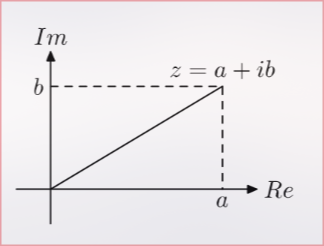
\includegraphics[scale=0.5]{img/pianoArgandGauss.png}
  \caption{Piano di Argand-Gauss}
  \label{fig:image}
\end{figure}
Essendo gli assi ortogonali $|a + ib|$ è la distanza dal punto $(a,b)$ dall'origine nel piano cartesiano
\\ \\
Dati due numeri complessi $z$ e $w$, il modulo $|z - w|$ è la distanza tra i punti corrispondenti a $z$ e $w$
\\ \\
Sia $r$ un numero reale positivo. Nel piano di Gauss l'insieme $\{z \in \mathbb{C} | | z - z_0 | < r\}$ rappresenta i punti interni alla circonferenza di centro $z_0$ e raggio $r$
\\ \\
I punti della circonferenza di equazione $x^2 + y^2 = 1$ (centro origine e raggio 1), corrispondono ai numeri complessi $\cos \vartheta + i \sin \vartheta$, con $\vartheta \in [0, 2k\pi]$
\\ \\
Sia $z \neq 0 \in \mathbb{C}$ e consideriamo: 
\\ \\
$z' = \frac{z}{|z|} = c + di$ si ha $|z'| = \sqrt{c^2 + d^2} = 1$
\\ \\
Esiste un numero reale $\vartheta$ (unico se lo richiediamo in $[0, 2k\pi]$) tale che $z' = \cos(\vartheta) + i\sin(\vartheta)$ e si ha $|z|z'$ da cui 
\\ \\
$z = |z|(\cos(\vartheta) + i\sin(\vartheta)) \rightarrow$ \textbf{Rappresentazione Trigonometrica}
\\ \\
$\vartheta$ è l'angolo formato dalla semiretta per $z$ uscente dall'origine e la semiretta positiva dell'asse orizzontale 
\\ \\
$\vartheta$ è detto argomento del numero complesso $z \neq 0$ (ed è determinato da $z$ a meno di multipli di $2k\pi$).
\\ \\ 
Si indica con $Arg(z)$
\section{Richiami di Trigonometria}
\begin{figure}[h]
  \centering
  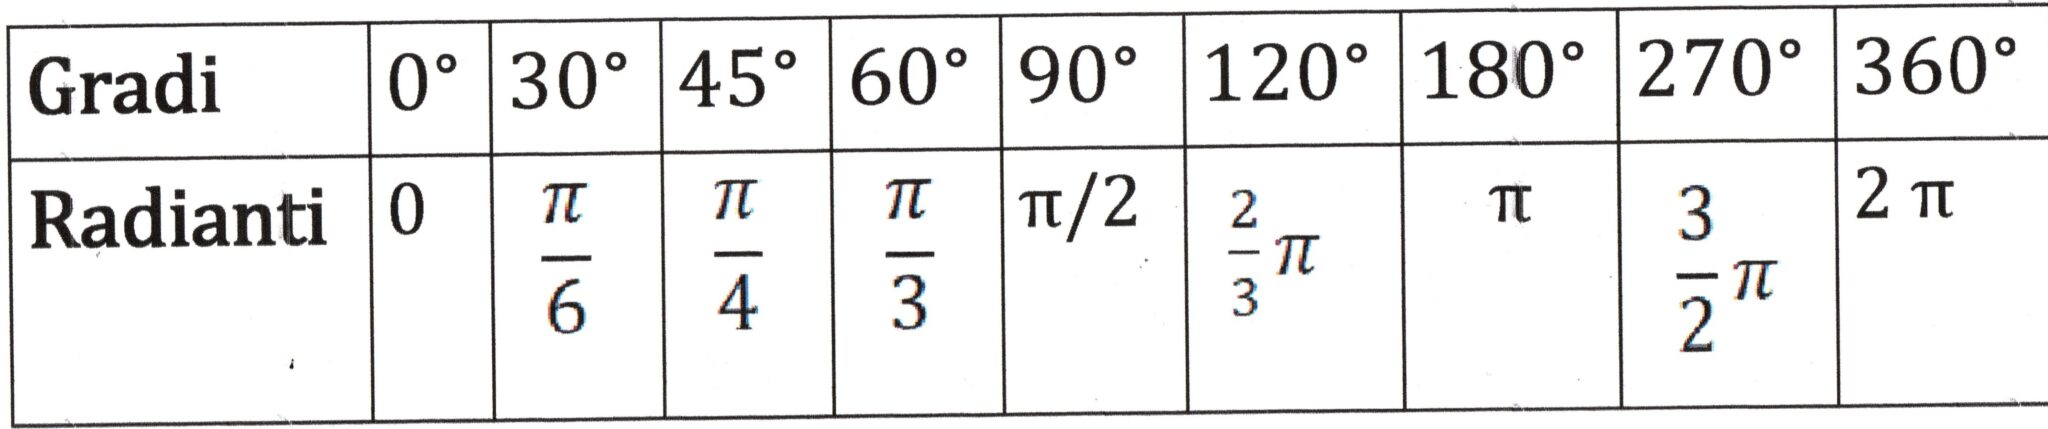
\includegraphics[scale=0.8]{img/tabellaGradiRadianti.jpg}
  \caption{Tabella di conversione gradi radianti}
  \label{fig:image}
\end{figure}

\section{Operazioni coi numeri complessi}
\subsection{Prodotto}
Se $z_1 = |z_1|(\cos(\vartheta) + i\sin(\vartheta))$ e $z_2 = |z_2|(\cos(\vartheta) + i\sin(\vartheta))$ sono numeri complessi non nulli, il loro prodotto è:
\\ \\
$z_1 z_2 = |z_1|(\cos(\vartheta) + i\sin(\vartheta)) |z_2|(\cos(\vartheta) + i\sin(\vartheta)) =  |z_1 z_2|(\cos(\vartheta_1 + \vartheta_2) + i\sin(\vartheta_1 + \vartheta_2))$
\\ \\
Pertanto:
\begin{itemize}
    \item{$|z_1z_2| = |z_1| |z_2|$}
    \item{Arg($z_1z_2$) = Arg($z_1$) + Arg($z_2$)}
\end{itemize}
Per definizione $i = \sqrt{-1}$
\mprop{Valore di i}{$i = \sqrt{-1} \iff i^2 = -1$}
\cor{}{Un prodotto tra due numeri complessi può risultare in un numero reale}
\subsection{Potenze}
Se $z_1 = |z_1|(\cos(\vartheta_1) + i\sin(\vartheta_1))$ allora:
\\ \\
$z_1^2 = |z_1|^2(\cos(\vartheta_1)^2 + i\sin(\vartheta_1)^2)$ \\
$z_1^3 = |z_1|^3(\cos(\vartheta_1)^3 + i\sin(\vartheta_1)^3)$ \\
$\dots$ \\
$z_1^n = |z_1|^n(\cos(\vartheta_1)^n + i\sin(\vartheta_1)^n)$ \\ \\
Pertanto:
\begin{itemize}
    \item{$|z_1^n| = |z_1|^n$}
    \item{Arg($z_1^n$) = nArg($z_1$)}
\end{itemize}
Di conseguenza, sappiamo calcolare le radici:
\\ \\
Per $z_0 \neq 0$ e $n \geq 1$ si ha 
\\ \\
$z^n = z_0$
\\ \
Se, e solo se, $|z|^n = |z_0|$ e $n\vartheta_0 + 2k\pi$ al variare di $k \in \mathbb{Z}$, ove $\vartheta =$ Arg($z$) e $\vartheta_0 =$ Arg($z_0$)
\mprop{formula di de Moivre}{$z^n = z_0 \Longleftrightarrow
\begin{cases}
|z| = \sqrt[n]{|z_0|} \\Complesso
\vartheta = \frac{\vartheta_0}{n} + \frac{2k\pi}{n} \quad k = 0, \dots, n-1
\end{cases}$}
Ci sono $n$ radici $n$-esime distinte per ogni numero complesso diverso da $0$, che fomrano i vertici di un $n$-gono regolare centrato nell'origine 
\mprop{Esponenziale complesso}{Sia $z = x + iy$, con $x$ e $y$ reali, e poniamo \\ \\
$e^z = e^{x + iy} = e^x(\cos y + i \sin y)$}
Al variare di $z \in \mathbb{C}$, $e^z \neq 0$ e si ha $e^{z + w} = e^z e^w$
\\ \\
Per ogni numero complesso $z_0 = |z_0|(\cos(\vartheta_0) + i\sin(\vartheta_0) \neq 0$ si ha:
\\ \\
$z_0 = |z_0|e^{i\vartheta_0} = pe^{i\vartheta_0} \rightarrow$ \textbf{Rappresentazione Esponenziale} \\ \\
Ove $\vartheta_0$ è l'argomento di $z_0$ e $p = |z_0|$
\qs{Risoluzione di un equazione utilizzando la notazione esponenziale}{Dato $z \in \mathbb{C}$ trova le soluzioni di $z^2 * \overline{z} = z$}
\sol{$z^2 = r^2e^{i2\vartheta}, \overline{z} = re^{-i\vartheta}, z = re^{i\vartheta}$ abbiamo quindi:
\\ \\
$r^2e^{i2\vartheta} re^{-i\vartheta} = re^{i\vartheta}$
\\ \\
moltiplichiamo r a primo membro e otteniamo 
\\ \\
$r^3e^{i2\vartheta} e^{-i\vartheta} = re^{i\vartheta}$
\\ \\
svolgiamo i calcoli in e a primo membro raccogliendo i e otteniamo:
\\ \\
$r^3e^{i(2\vartheta - \vartheta} = re^{i\vartheta}$
\\ \\
$r^3e^{i\vartheta} = re^{i\vartheta}$
\\ \\ 
dividiamo per $e^{i\vartheta}$
\\ \\Complesso
$r^3 = r$
\\ \\ 
otteniamo quindi:
\\ \\
$r^3 - r = 0$ \\ \\
$r(r^2 - 1)$ \\ \\
otteniamo quindi
$r=+-1$ e $r=0$
}
\mprop{Identità di Eulero}{$e^{i\pi} + 1 = 0$}
I numeri complessi sono un campo algebricamente chiuso. Vale il cosidetto 
\thm{Teorema fondamentale dell'algebra}{Sia $P(X$ un polinomio di grado posittivo in $\mathbb{C}[X]$. Allora esiste un numero complesso $z_0$ tale che $P(z_0) = 0$}
Ogni polinomio a coefficienti in $\mathbb{R}$ si fattorizza come prodotto di polinomi lineari $X - \alpha$ con $\alpha \in \mathbb{R}$ e polinomi di grado due $(X - \beta)(X - \overline{\beta})$ con $\beta \in \mathbb{C}$
\section{Interpretazione Geometrica}
Le operazioni in $\mathbb{C}$ hanno una rappresentazione geometrica nel piano di Gauss
\begin{figure}[h]
 \centering
  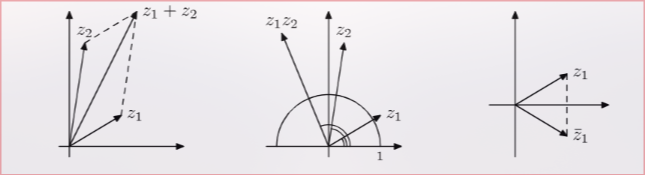
\includegraphics[scale=0.5]{img/interpretazioneGeometricaSuPianoDiGauss.png}
  \caption{Interpretazione Geometrica su Piano di Argand-Gauss}
  \label{fig:image}
\end{figure}
La somma per un numero $z_2$ è la traslazione corrispondente a quel vettore. \\ \\
Il prodotto per un numero $z_2 = pe^{i\alpha} \neq 0$ è una dilatazione di rapporto $p$ seguita da una rotazione di angolo $\alpha =$Arg($z_2$)
\chapter{Spazi Vettoriali}
\dfn{Spazi Vettoriali}{Uno spazio vettoriale su $K$ è un insieme non vuoto $V$ dotato di due operazione (Moltiplicazione e Addizione)}
$+ : K \varprod K \rightarrow V$
\\ \\
$* : K \varprod K \rightarrow V$
\section{Proprietà degli spazi vettoriali}
\begin{itemize}
    \item{$(u + v) + w = v + (u + w) \forall u, v \in V$}
    \item{$u + v = v + u \forall u, v \in V$}
    \item{$\exists \ \Vec{o} \in V : v + \Vec{o} = \Vec{o} + v \forall u, v \in V$}
    \item{$\forall v \in V$ esiste un vettore indicato come $-v$ tale che: $v + (-v) = 0$}
    \item{$(\alpha * \beta) * v = \alpha * (\beta * v) \forall \alpha,\beta \in K \forall u, v \in V$}
    \item{$\alpha + \beta) * v = \alphav + \betav \forall \alpha,\beta \in K \forall u, v \in V$}
    \item{$1 * v = v \forall v \in V$}
\end{itemize}
\section{Vettori Geometrici}
Vettori geometrici anche detti segmenti orientati sono rappresentazioni dei vettori su un piano $\mathbb{R}^2$ o $\mathbb{R \varprod C}$ 
\begin{figure}[h]
 \centering
  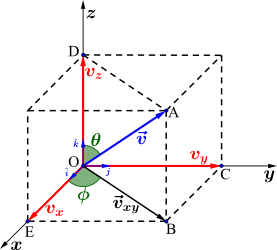
\includegraphics[scale=0.5]{img/vettoreSulPiano.png}
  \caption{Vettore sul piano}
  \label{fig:image}
\end{figure}
\textbf{Proprietà}
\begin{itemize}
    \item{$\Vec{v} + \Vec{v} = 2\Vec{v}$}
    \item{$V = K$ Spazio vettoriale su $K$}
    \item{$K$ campo, $V = L$ un altro campo tale che $V \subset K$ \\ \\
    Esempi: \\ \\
    $K = \mathbb{Q} \subset \mathbb{R} = L ; K = \mathbb{R} \subset \mathbb{C} = L$
    \\ \\
    $V$ è uno spazio vettoriale su $K$}
    \item{$V = K^m = \{a_1, a_2, \dots, a_m\} | a_1, a_2, \dots, a_m \in K$ \\ \\
    $(a_1, a_2, \dots, a_m) + (b_1, b_2, \dots b_m) = (a_1 + b_1, a_2 + b_2, \dots a_m + b_n)$ e si scrive $\begin{pmatrix}
a_1 \\
a_2 \\
a_3 \\
\vdots
\end{pmatrix}
+
\begin{pmatrix}
b_1 \\
b_2 \\
b_3 \\
\vdots
\end{pmatrix}
=
\begin{pmatrix}
a_1 + b_1 \\
a_2 + b_2 \\
a_3 + b_3 \\
\vdots
\end{pmatrix}

\lambda \in \mathbb{K}, \quad
\begin{pmatrix}
a_1 \\
a_2 \\
\vdots \\
a_m
\end{pmatrix}
\in V = \mathbb{K}^M \quad \text{definisco} \quad \lambda \cdot
\begin{pmatrix}
a_1 \\
a_2 \\
\vdots \\
a_m
\end{pmatrix}
=
\begin{pmatrix}
\lambda a_1 \\
\lambda a_2 \\
\vdots \\
\lambda a_m
\end{pmatrix}
$}
\item{
$V = $ insieme dei polinomi in $x$ con coefficienti in $K$ e si scrive $K[x]$ il quale è uno spazio vettoriale
}
\item{$V =$ insieme di funzioni da $R \rightarrow R$ e anch'esso rappresenta uno spazio vettoriale}
\end{itemize}

\end{document}
